\documentclass{beamer}
\usepackage[english]{babel}
\usepackage{amsmath,graphicx}

%%%%%%%%%% Start TeXmacs macros
\newcommand{\mathd}{\mathrm{d}}
\newcommand{\nospace}{}
\newcommand{\tmmathbf}[1]{\ensuremath{\boldsymbol{#1}}}
\newcommand{\tmop}[1]{\ensuremath{\operatorname{#1}}}
%%%%%%%%%% End TeXmacs macros

\begin{document}

{\screens{\begin{frame}
  \
  
  \
  
  \
  
  \
  
  \
  
  \title{计算视觉与模式识别}
  
  \maketitle
  
  \ 
\end{frame}}{\frametitle{黑体辐射}

{\hspace{3em}}\resizebox{0.7\columnwidth}{!}{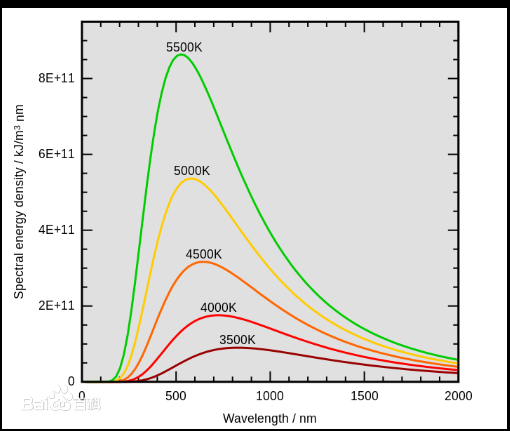
\includegraphics{img/black_body_radiators.png}}}{\begin{frame}
  \
  
  \qquad\resizebox{0.8\columnwidth}{!}{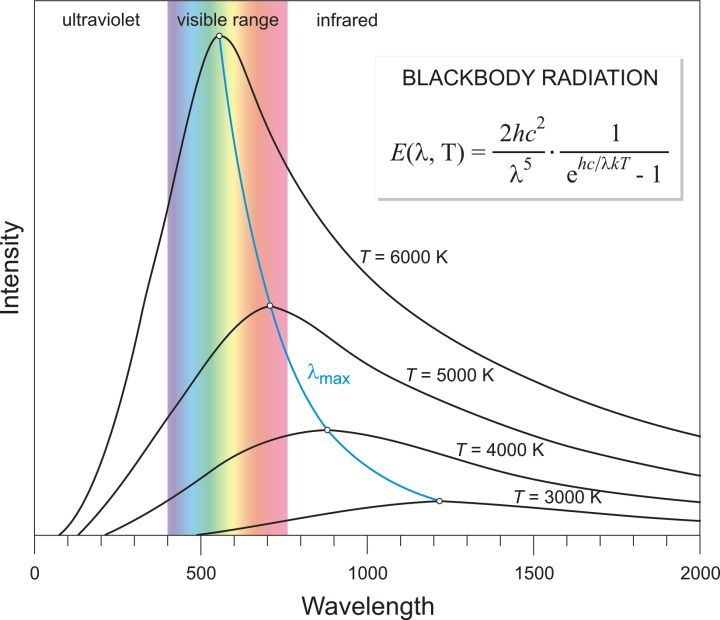
\includegraphics{img/black_body_radiators_color.jpg}}
\end{frame}}{\begin{frame}
  \frametitle{太阳与天空}
  
  {\hspace{4em}}\resizebox{0.7\columnwidth}{!}{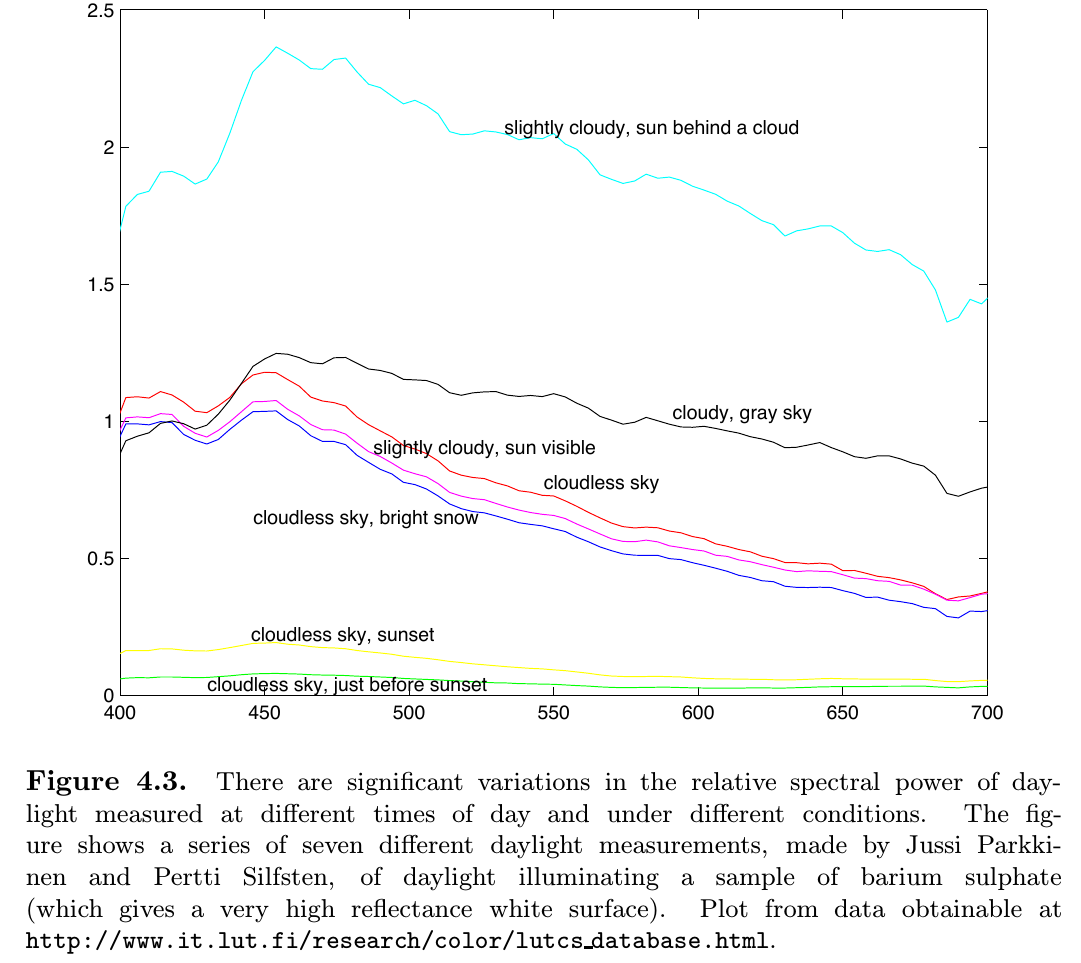
\includegraphics{img/day_light.png}}
\end{frame}}{\begin{frame}
  \frametitle{灯光}
  
  \qquad\resizebox{0.8\columnwidth}{!}{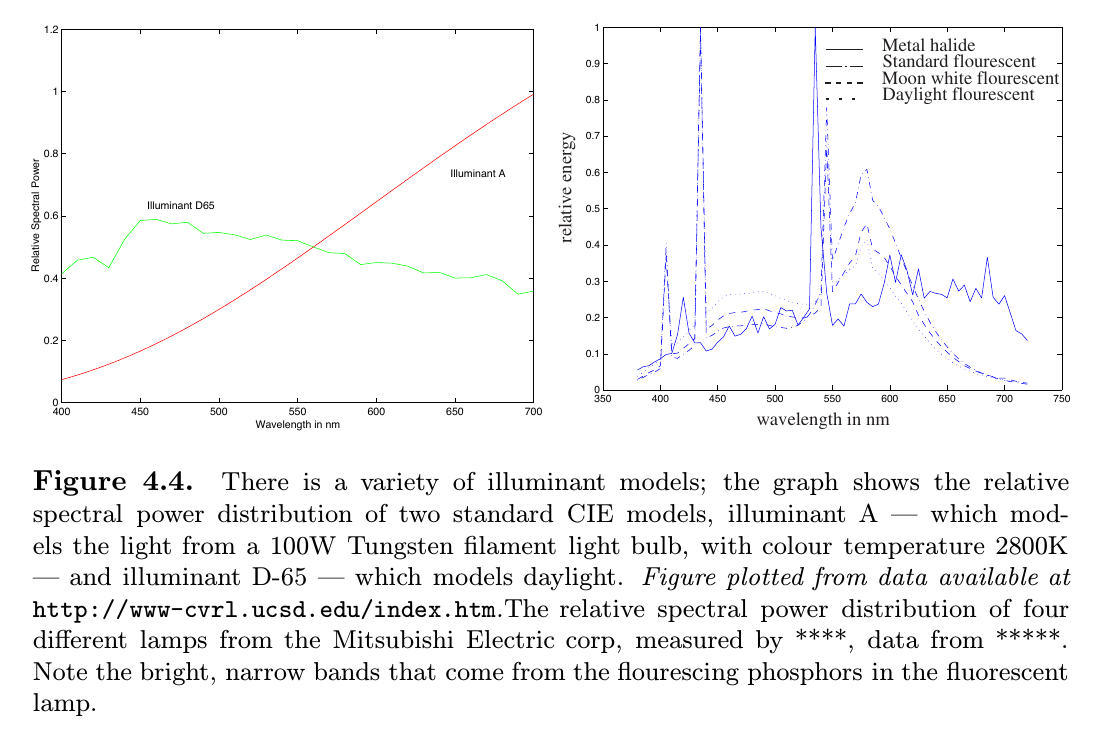
\includegraphics{img/illuminant_models.png}}
\end{frame}}{\begin{frame}
  \frametitle{表面的颜色}
  
  朗伯加镜面反射模型:
  \begin{eqnarray*}
    E (\lambda) & = & \rho_{\tmop{dh}} (\lambda) S (\lambda) \times
    \text{geometric terms} + \text{specular terms}
  \end{eqnarray*}
\end{frame}}{\begin{frame}
  \frametitle{光谱反射率------花与叶}
  
  \qquad\resizebox{0.9\columnwidth}{!}{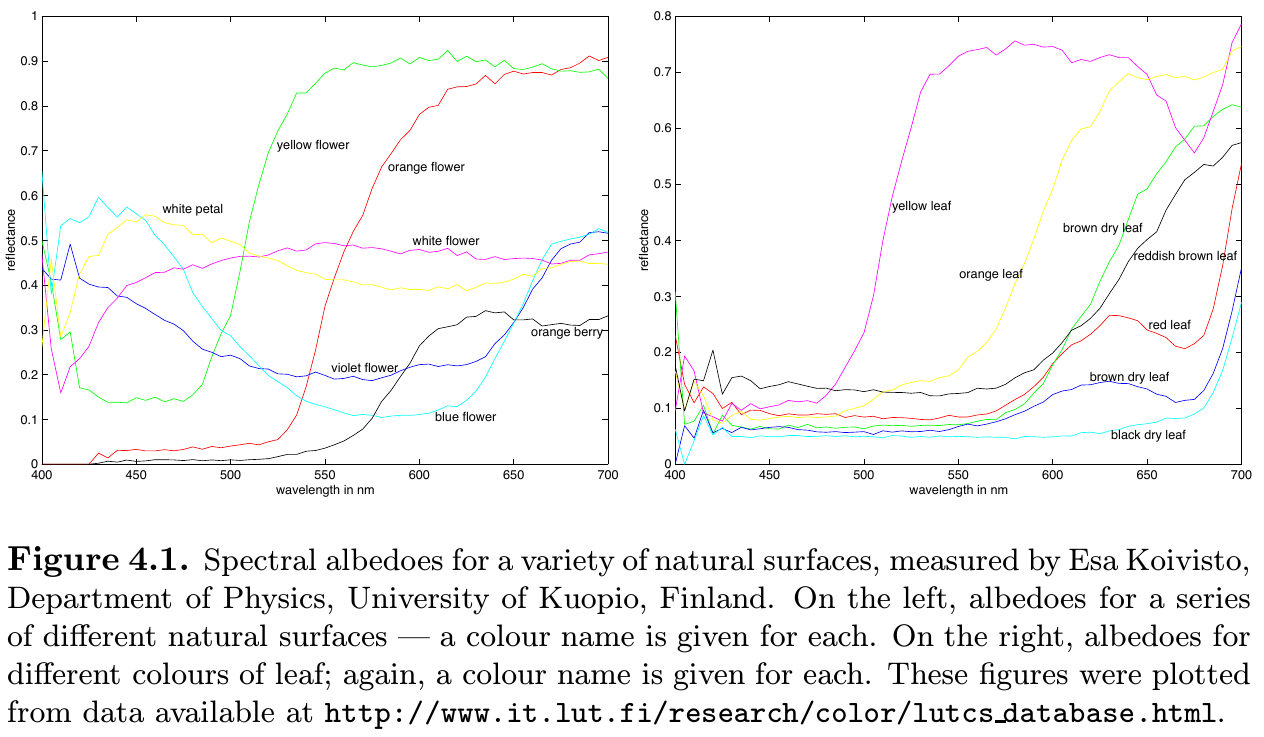
\includegraphics{img/spectral_albedoes_for_surfaces.png}}
\end{frame}}{\begin{frame}
  \frametitle{光谱反射率------红花与绿叶}
  
  \quad\resizebox{0.9\columnwidth}{!}{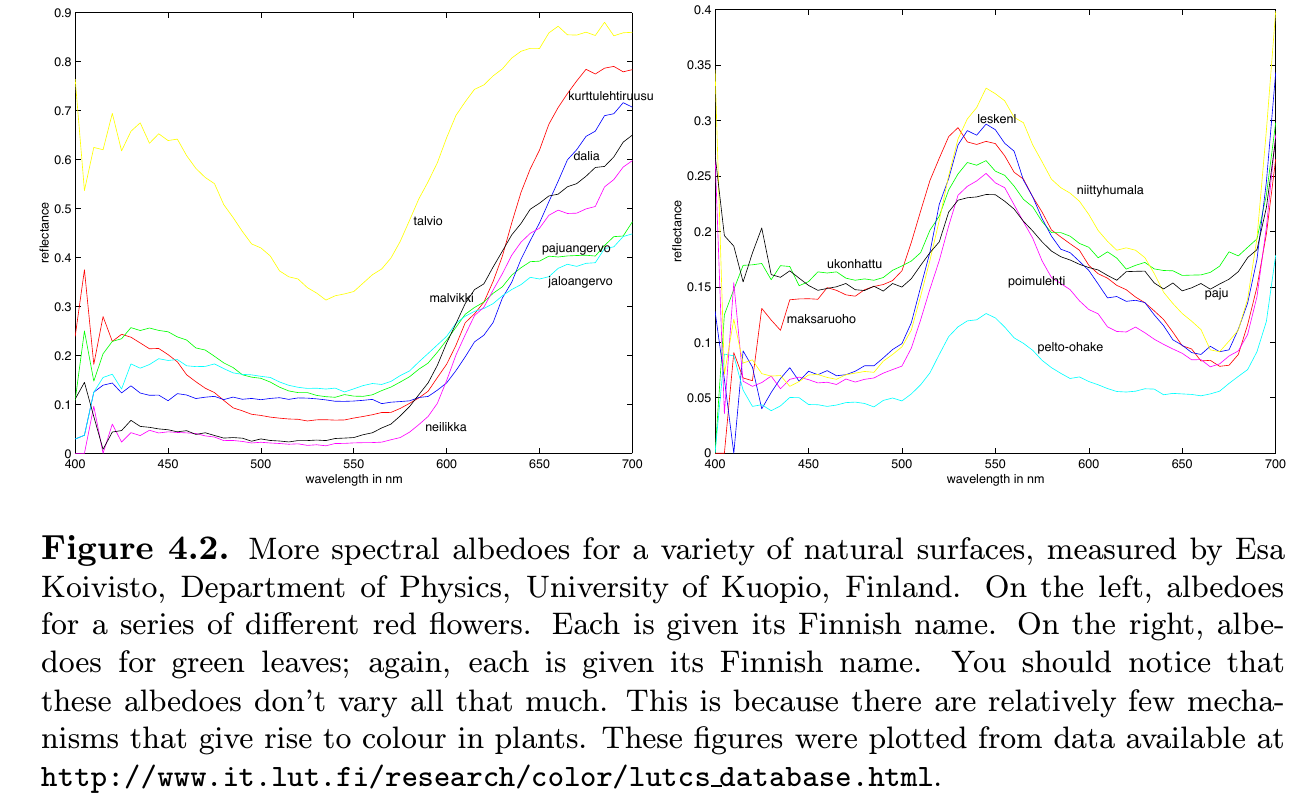
\includegraphics{img/more_spectral_albedoes_for_surfaces.png}}
  
  \ 
\end{frame}}{\begin{frame}
  \frametitle{颜色匹配}
  
  \quad\resizebox{0.9\columnwidth}{!}{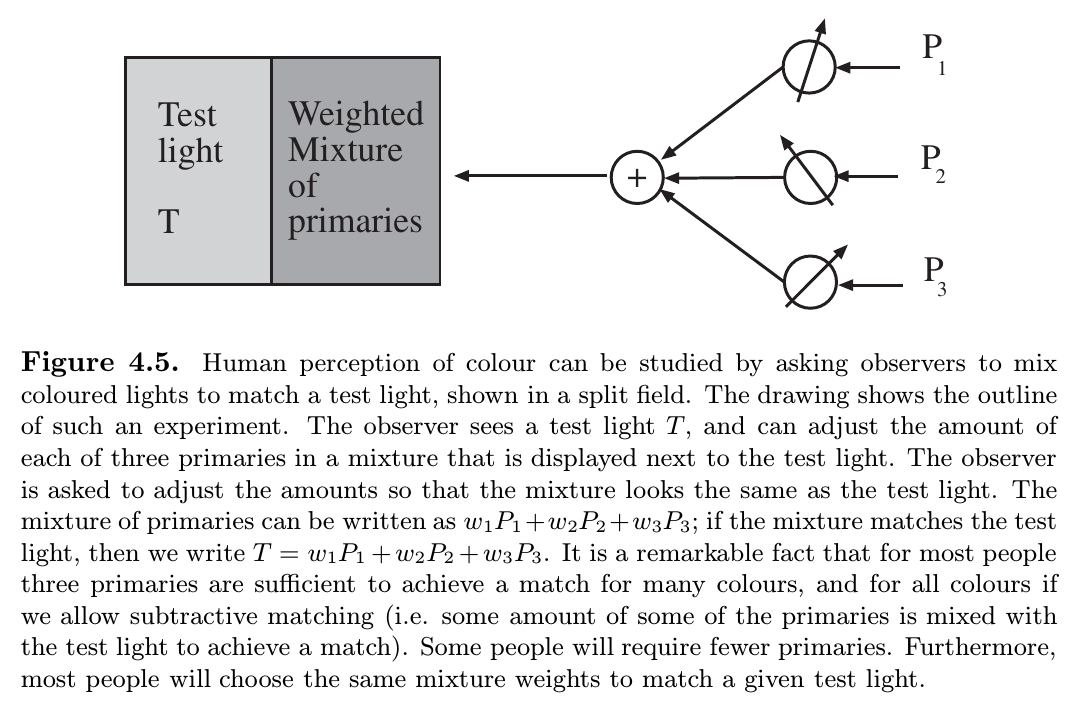
\includegraphics{img/color_match.png}}
\end{frame}}{\begin{frame}
  \frametitle{Grassman 定律}
  \begin{eqnarray*}
    T (\tmmathbf{w}) & = & \sum_i w_i P_i\\
    T (\tmmathbf{v}) & = & \sum_i v_i P_i\\
    T (k\tmmathbf{w}) + T (k\tmmathbf{v}) & = & k \nospace T
    (\tmmathbf{w}+\tmmathbf{v})
  \end{eqnarray*}
\end{frame}}{\begin{frame}
  \frametitle{颜色感受体}
  \begin{eqnarray*}
    p_k & = & \int_{\Lambda} \sigma_k (\lambda) E (\lambda) \mathd \lambda
  \end{eqnarray*}
  
\end{frame}}{\begin{frame}
  \frametitle{彩色视觉}
  
  \resizebox{364pt}{180pt}{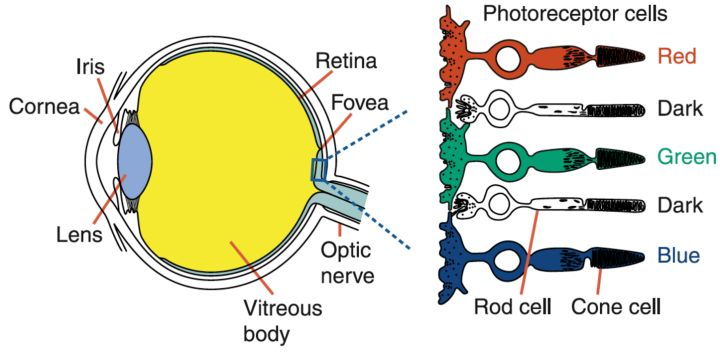
\includegraphics{img/human_eye_color_vision.jpg}}
\end{frame}}{\begin{frame}
  \frametitle{视锥细胞响应曲线}
  
  \quad\resizebox{0.9\columnwidth}{!}{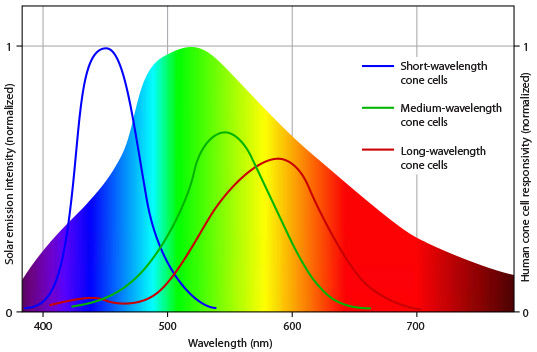
\includegraphics{img/cone_cell_response.jpg}}
\end{frame}}}

\end{document}
